\documentclass[../Main/Knit.tex]{subfiles}


\section{RNA Extraction}
\label{section: ch2_rna_extraction}
Total RNA from mouse entorhinal cortex was extracted by Dr. Isabel Castanho using the AllPrep DNA/RNA Mini Kit (Qiagen). Samples were selected for long-read sequencing based on RNA quality and quantity, previously determined using RNA ScreenTape assay (Agilent) on 2200 TapeStation System or the RNA 6000 Nano kit (Agilent) on the 2100 Bioanalyzer (Section \ref{section:ch2_bioanalyzer}). 


\section{Polymerase Chain Reaction (PCR)}
\label{section:ch2_PCR_explanation} 
To generate sufficient DNA for sequencing, single-stranded DNA was amplified using Polymerase Chain Reaction (PCR\nomenclature{PCR}{Polymerase Chain Reaction}), a well-established method of generating multiple copies of the same DNA sequence. Mimicking natural DNA replication, this relies on a thermostable DNA polymerase, a set of primers specific to the region of interest, and a cocktail of various other components required for polymerisation (deoxynucleotides\nomenclature{dNTPs}{Deoxynucleotides} , buffers). This reaction is then subjected to a series of heating and cooling steps: 
\begin{enumerate}
	\item Denaturation at 96C, to separate any double-stranded DNA 
	\item Annealing, typically between 55 to 65C, for the binding of primers to the complementary sequences on the single-stranded DNA; the specific annealing temperature is dependent on the primer sequence. 
	\item Extension at 72C to allow the polymerase to extend the primers, consequently synthesising a new complementary DNA strand using dNTPs
\end{enumerate} 
These three steps are then repeated for a number of times, "cycles", for an exponential generation of the DNA template of interest.

Single-stranded DNA generated from SMARTer PCR synthesis kit in the official Iso-Seq protocol was amplified by PCR using PrimeSTAR GXL DNA Polymerase (ClonTech). Also performed for targeted sequencing. 


\section{Agarose Gel Electrophoresis}
\label{section:ch2_agarose_explanation}  
Agarose gel electrophoresis allows the separation of (double-stranded) DNA molecules based on its length. It is most commonly used to determine DNA quality and quantity, and assess the efficiency of molecular biology techniques such as PCR amplification. It works on the principle that by applying an electrical charge, negatively-charged DNA migrates through a gel matrix towards the positive anode at a rate dependent on DNA size: smaller DNA fragments migrate faster, and thus move further through the gel within a specific time frame. The separated DNA can be then visualised using a fluorescent dye that intercalates into the DNA structure and fluoresces under ultraviolet light. 

For this thesis, visualisation of DNA through gel electrophoresis was required primarily for optimising the number of PCR cycles for amplification, and for validating transcripts identified from Iso-Seq in Chapters X. A 1.5\% agarose gel was made, with the separated DNA visualised using ethidium bromide on XXXX, as detailed in Section \ref{Isoseq_Protocol_running_agarose_gel}.

\section{Bioanalyzer and Tapestation}
\label{section:ch2_bioanalyzer} 
ScreenTape and Bioanalyzer assays are commonly used to provide accurate assessment of nucleic acid quality and size, prior to proceeding with downstream experiments. As an automative alternative to agarose gel electrophoresis, both assays similarly take advantage of nucleic acid's inclination to migrate in response to an electrical field.
While the Bioanalyzer assay is more sensitive than the ScreenTape assay, it is more expensive to run as it uses a chip consisting of 12 sample wells rather than independent lanes on the ScreenTape. 

For this thesis, most of the assessments of DNA quality in the Iso-Seq and ONT protocol were performed on the DNA 12000 Kit (Agilent) on the 2100 Bioanalyzer assay for accurate determination of library molarity (Section X). However, the D5000 ScreenTape (Agilent) was used in a few of the quality control steps where it is optional to assess for DNA quality (Section X).

RNA extracted by Dr Isabel Castanho was also run on RNA ScreenTape assay and the Bioanalyzer RNA analysis to provide accurate evaluation of RNA degradation; this is represented by a RNA Integrity Number (RIN\nomenclature{RIN}{RNA Integrity Number}) between 1 and 10, where 1 is indicative of high degradation, and 10 of low degradation and thus high integrity (Figure \ref{fig:bionalayzer_pics}). As a pre-requisite for good sequencing yield on Sequel and MinION, only samples with RIN $>$ 8 were selected for long-read sequencing on Iso-Seq and ONT protocol.

\spacetable
\begin{figure}[h]
	\centering
	\begin{subfigure}{0.4\linewidth}
		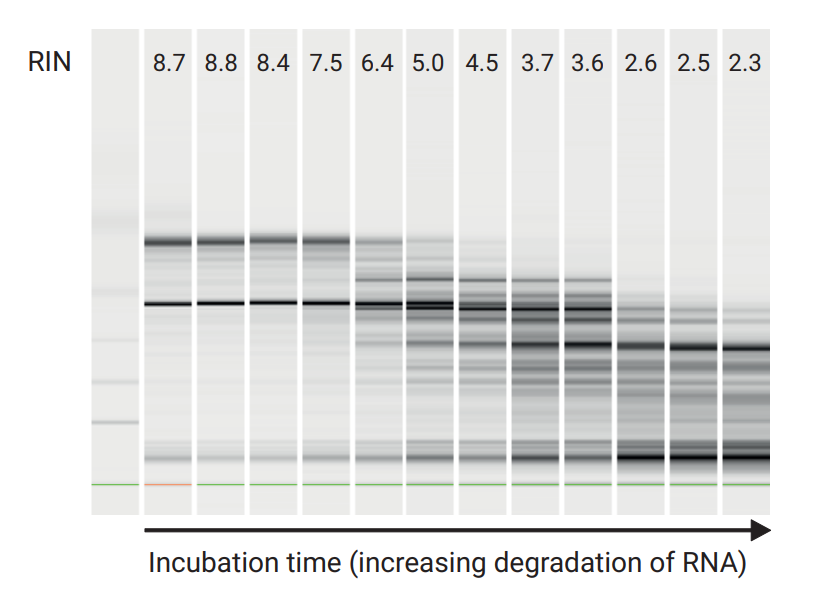
\includegraphics[width=\linewidth, height=0.21\textheight]{Pictures/RNA_degradation.png}
		\caption{Automated gel electrophoresis of RNA degradation}
	\end{subfigure}
	\hspace{2em}
	\begin{subfigure}{0.4\linewidth}
		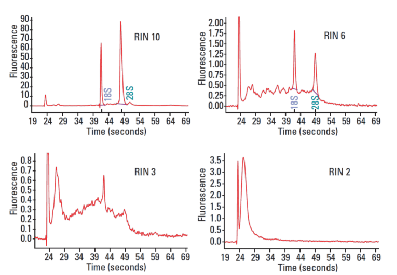
\includegraphics[width=\linewidth, height=0.21\textheight]{Pictures/RIN_range.png}
		\caption{Electropherogram of RNA degradation}
	\end{subfigure}
	\hspace{2em}
	\begin{subfigure}{0.4\linewidth}
		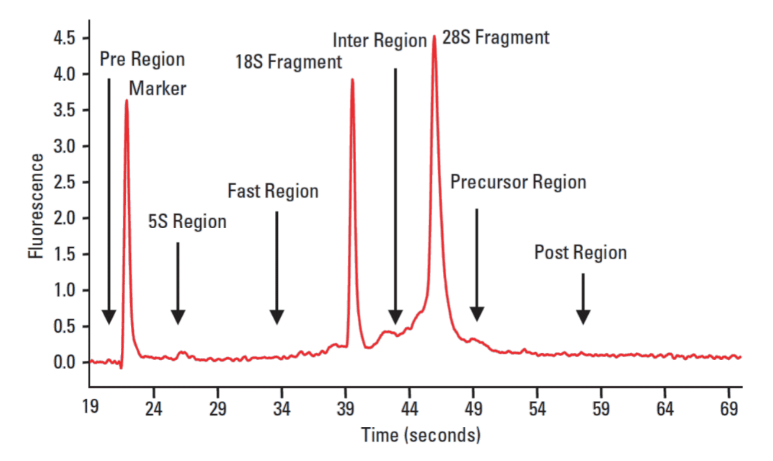
\includegraphics[width=\linewidth,
		height=0.21\textheight]{Pictures/RIN_regions.png}
		\caption{Electropherogram of regions that are indicative of RNA quality}
	\end{subfigure}
	\captionsetup{width=0.95\textwidth}
	\caption[Evaluation of RNA integrity with Bioanalyzer and Tapestation]%
	{\textbf{Evaluation of RNA integrity with Bioanalyzer and Tapestation}: Total RNA degradation can be observed by a shift towards shorter fragment size as depicted in Figure a, after prolonged incubation. The degree of degradation is represented by a RNA integrity number (RIN), ranging from intact (RIN = 10) to degraded (RIN = 2) RNA, and is calculated by the relative ratio of the fast region and 18S, 28S fragment (Figure c). Figures and legends are adapted from Mueller et al. 2016.}
	\label{fig:bionalayzer_pics}
	\end{figure} 

\section{Qubit}
\label{section:ch2_qubit}   
Qubit assays allow accurate nucleic acid quantification by the selective binding of fluorescent Qubit dyes to double-stranded DNA (dsDNA\nomenclature{dsDNA}{double-stranded DNA}) or RNA, making it more sensitive and specific than UV absorbance used in NanoDrop 8000 spectrophotometer (Thermo Fisher Scientific). It is commonly performed to determine the average concentration of DNA or RNA prior to proceeding with downstream experiments. Many of the steps in the Iso-Seq protocol and ONT protocol thus require performing Qubit assays, particularly post bead purification, and are detailed in Section \ref{Isoseq_Protocol_qubit}.  


\pagebreak
\section{Target Capture using IDT Probes}
For gene enrichment in targeted sequencing, the official PacBio protocol “cDNA Capture Using IDT
xGen® Lockdown Probes” was used, with minor changes adapted from the official IDT protocol “xGen hybridisation capture of DNA libraries”, as outlined in Figure X. In brief, the samples with unique non-overlapping barcodes were pooled in equal molarity post ampure bead purification and hybridised with target-specific probes; the captured cDNA was then washed with multiple wash buffers, amplified and purified with AMPure beads.   Pooling 6 – 9 libraries prior to target capture simplifies laboratory workflow and minimises associated sequencing costs. 


